
\chapter{INTRODUCTION}
Experimenting with the available typographic conventions defined in the Purdue file: \NL \Literal|pa-typographic-conventions.sty|:  these include \Emph{Emph} \First{First} \First{Title} \Keys{Keys} \Literal|Literal| \Menu{Menu} \Menu{Open menu > Preferences} \Shell{Shell.sh}. Now let's try out a footnote\footnote{I'm a footnote!}, one of the fancy TODO notes  \todocomment{Do I really need this?}, and more scary TODO \todowarn{Be careful here}, as well as a a todo error \todoerror{This is wrong!} as well as a citation \cite{Howell:1984_HaloOrbits}. Note the TODO comments currently only show up in \Literal|quick| or \Literal|debug| modes (for now).


\section{Subcaption / Cleveref Testing}
Here is a very important and informative figure for Orion. You can see in \cref{fig:orion} that there is both \cref{fig:orion:a} and \cref{fig:orion:b}! There is also important information in \cref{tab:sample_table}. If you're confused, then \cref{eq:euler} should clarify things. Some other ways to put it: \cref{eq:euler,eq:pythagorean} and \cref{eq:euler,eq:pythagorean,eq:calculus}. 

\begin{figure}[p]
    \centering
    \begin{subcaptionblock}{.49\textwidth}
        \centering
        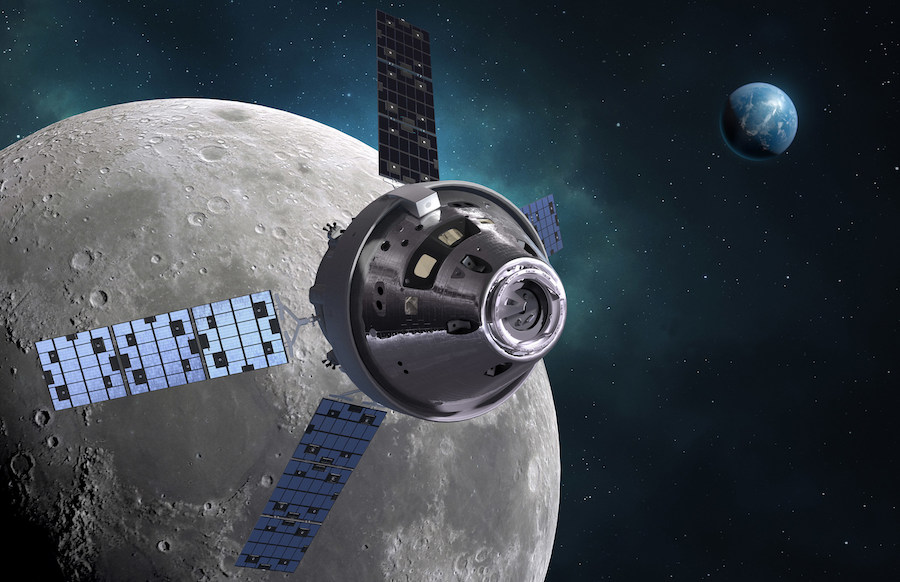
\includegraphics[width=\textwidth]{orion1}
        \caption{Orion 1}
        \label{fig:orion:a}
    \end{subcaptionblock} %
    \begin{subcaptionblock}{.49\textwidth}
        \centering
        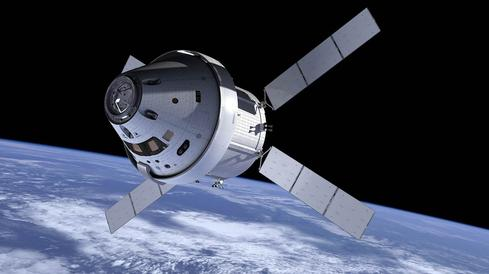
\includegraphics[width=\textwidth]{orion2}
        \caption{Orion 2}
        \label{fig:orion:b}
    \end{subcaptionblock} %
    \caption{Two images of Orion: \subref{fig:orion:a} and \subref{fig:orion:b}.}
    \label{fig:orion}
\end{figure}

\begin{table}[p]
    \centering
    \caption{Sample Table}
    \begin{tabular}{|c|c|}
    \hline
        Sample & Table\\
        $\xNd$ & 2\\
    \hline
    \end{tabular}
    \label{tab:sample_table}
\end{table}

\subsection{Important Math}

\begin{equation}
    e^{i\pi}+1=0
    \label{eq:euler}
\end{equation}

\begin{equation}
    a^2+b^2=c^2
    \label{eq:pythagorean}
\end{equation}

\begin{equation}
    \frac{df}{dt} = \lim_{h\rightarrow 0} \frac{f(t+h)-f(t)}{h}
    \label{eq:calculus}
\end{equation}

\subsection{Numbers/Units}
Some of the number formats available: \num{-e10}. \numproduct{2 x 4}. \numrange{10}{11}. \ang{12.3}.

Experimenting with the siunits package: 8 \unit{\kilo\gram\metre\per\square\second}. 9\unit{\newton}. \qty{2.3e27}{\kilogram}. \qty[per-mode = fraction]{1,345}{\coulomb\per\mole}.

\subsubsection{A subsubsection} 
A subsubsection for testing out the table of contents

\paragraph{A paragraph}
What happens for a paragraph in the table of contents?

\subsection{Custom variables}

Variables can be defined as functions in \Menu{t0-template > te4-custom-variables.tex}

The rotating $\xNd$ axis is clearly the best of all axes. But even better is the $\vectorFmt{\xNd}$ vector and the $\unitVecFmt{\xNd}$ direction! See the appenix in Debug mode for details

\subsection{Custom colors}
There are a variety of available colors from Purdue's branding\footnote{see \href{https://marcom.purdue.edu/our-brand/visual-identity/}{https://marcom.purdue.edu/our-brand/visual-identity/}} like: {\color{purdue-boilermaker-gold} Boilermaker Gold}, {\color{purdue-rush} Rush}. This example document also include the Tableau colors\footnote{used in matplotlib - \href{https://matplotlib.org/3.4.1/gallery/color/named_colors.html}{https://matplotlib.org/3.4.1/gallery/color/named\_colors.html}}. For example, {\color{tab-blue} tab-blue} and {\color{tab-red} tab-red}.

\subsection{Acronyms}
Acronyms handled through \verb|glossaries|, and defined in \Menu{t0-template > te6-acronyms.tex}. For example, the first time we will refer to the \gls{crtbp}, and in the future only say \gls{crtbp}.
